% Relativistic Chapter XI, §102–103: Continuous Velocity/Density Variation KH
% Relativistic generalization of Chandrasekhar, Chapter XI §102–103
% Conventions: see RELATIVISTIC_CONVENTIONS.md

\chapter{Relativistic Kelvin--Helmholtz Instability with Continuous Profiles}
\label{ch:rel-11-KH-cont}

%% ================================================================
\section{The effect of a continuous variation of $U$ on the relativistic
  Kelvin--Helmholtz instability}\label{sec:rel-102}

\subsection{Motivation and setup}

In the non-relativistic theory (\S\,102 of the classical treatment),
the Kelvin--Helmholtz instability at a sharp interface is independent
of the magnitude of the velocity jump $|U_{1}-U_{2}|$.  One introduces
a transition layer in which $U$ varies continuously, and discovers that
the Richardson number governs stability.  In the relativistic regime
the energy stored in the bulk motion contributes to the inertia, and
Lorentz factors modify the effective shear.  In this section we
construct the relativistic analogue of the transition-layer problem.

\subsubsection{Physical contexts}
Relativistic velocity shear with continuous profiles arises in:
\begin{enumerate}
\item \textbf{Astrophysical jets.}  The boundary layer between a
  relativistic jet (bulk Lorentz factor $\Lf_{\mathrm{jet}}\gg 1$) and
  the ambient medium is a smooth shear layer whose stability controls
  jet collimation and entrainment.
\item \textbf{Gamma-ray burst outflows.}  The interface between the
  fast ejecta and the slower cocoon develops a velocity profile that is
  smoothed by relativistic viscosity on a scale set by the
  BDNK viscous transport coefficients \citep{Bemfica2018,Kovtun2019}.
\item \textbf{Heavy-ion collisions.}  The quark--gluon plasma fireball
  exhibits strong longitudinal velocity gradients; its stability against
  Kelvin--Helmholtz-type modes affects the development of flow
  anisotropies.
\end{enumerate}

\subsubsection{Background flow}
We work in the frame of the transition layer.  The unperturbed flow is
planar: $U^{\mu}=(U^{0},U(z),0,0)$ with $U(z)$ the $x$-directed
streaming velocity.  The metric is Minkowski, $\eta_{\mu\nu}=
\mathrm{diag}(-1,+1,+1,+1)$, with $c$ kept explicit.

Define the local Lorentz factor
\begin{equation}
\label{eq:rel-11-102-1}
\Lf(z) = \frac{1}{\sqrt{1-U^{2}(z)/c^{2}}},
\end{equation}
so that the background four-velocity is
\begin{equation}
\label{eq:rel-11-102-2}
u^{\mu}_{0} = \Lf(z)\bigl(c,\,U(z),\,0,\,0\bigr).
\end{equation}

The relativistic enthalpy density is
\begin{equation}
\label{eq:rel-11-102-3}
\enthalpy = \frac{\varepsilon + p}{c^{2}},
\end{equation}
where $\varepsilon$ is the energy density (including rest-mass
contribution) and $p$ is the pressure.

\subsection{The three-layer profile}

Following the non-relativistic treatment, we adopt the profile
(cf.\ equation~\eqref{eq:11-43}):
\begin{equation}
\label{eq:rel-11-4}
\begin{aligned}
z > +d: &\quad \enthalpy = \enthalpy_{0}(1-\epsilon),
  &\quad U &= U_{0}, \\
+d > z > -d: &\quad \enthalpy = \enthalpy_{0},
  &\quad U &= U_{0}\,z/d, \\
z < -d: &\quad \enthalpy = \enthalpy_{0}(1+\epsilon),
  &\quad U &= -U_{0},
\end{aligned}
\end{equation}
where $\epsilon\ll 1$ parametrises the (small) enthalpy stratification.
In the relativistic context the natural stratification variable is the
enthalpy density $\enthalpy$, not the rest-mass density $\rho_{0}$,
because it is $\enthalpy$ that enters the relativistic Euler equation
and provides the inertia.

\paragraph{Causality constraint.}  The streaming velocity must satisfy
\begin{equation}
\label{eq:rel-11-5}
\boxed{|U_{0}| < c.}
\end{equation}
The corresponding Lorentz factor in the outer layers is
$\Lf_{0}=(1-U_{0}^{2}/c^{2})^{-1/2}$.

\subsection{Perturbation equations}

We consider linear perturbations about the background state.
Working in the ``relativistic Boussinesq'' approximation---retaining
the enthalpy stratification only in the buoyancy terms---the
linearised equation for the vertical displacement amplitude $\hat{w}$
of a normal-mode perturbation $\propto\exp[\mathrm{i}(k_{x}x+k_{y}y-\omega t)]$
takes the form (cf.\ equation~\eqref{eq:11-22}):
\begin{equation}
\label{eq:rel-11-6}
\enthalpy_{0}\,\Lf^{4}\!\left(\omega - k_{x}U\right)^{2}
\!\left[D^{2}\hat{w} - k^{2}\hat{w}\right]
- \enthalpy_{0}\,\Lf^{4}\!\left(\omega-k_{x}U\right)
k_{x}\frac{dU}{dz}\,D\hat{w}
- g\,k^{2}\frac{d\enthalpy}{dz}\,\hat{w} = 0,
\end{equation}
where $D=d/dz$, $k^{2}=k_{x}^{2}+k_{y}^{2}$, and the crucial
factor $\Lf^{4}$ (rather than the non-relativistic $1$) arises from
the relativistic enthalpy and the Lorentz boost of the effective
inertia in the sheared frame.

\paragraph{Origin of the $\Lf^{4}$ factor.}
The momentum equation for a relativistic perfect fluid reads
$\enthalpy\,u^{\nu}\nabla_{\nu}u^{\mu}=-\Delta^{\mu\nu}\partial_{\nu}p
+ \enthalpy\,g^{\mu}$, where $\Delta^{\mu\nu}=\eta^{\mu\nu}+
u^{\mu}u^{\nu}/c^{2}$ is the projection tensor.  When the background
has velocity $U(z)$ and we linearise, the Doppler-shifted frequency
$\tilde{\omega}=\omega-k_{x}U$ appears squared (from the material
acceleration $u^{\nu}\nabla_{\nu}$), and each power carries a Lorentz
factor from $u^{0}=\Lf c$, giving $\Lf^{2}\times\Lf^{2}=\Lf^{4}$.

\subsection{Boundary conditions}

Since $U$ is continuous at $z=\pm d$, the vertical displacement $\hat{w}$
is continuous there.  At each interface the jump condition becomes the
relativistic analogue of equation~\eqref{eq:11-45}:
\begin{equation}
\label{eq:rel-11-7}
\Delta_{\pm d}\!\biggl[
  \enthalpy\,\Lf^{4}\!\left(\omega-k_{x}U\right)
  \!\left(\frac{dU}{dz}\right)\hat{w}
\biggr]
- g\,k^{2}\,\Delta_{\pm d}(\enthalpy)\,\hat{w}_{\pm d} = 0.
\end{equation}

\subsection{Solutions in the three regions}

In each region of constant $\enthalpy$, equation~\eqref{eq:rel-11-6}
reduces to the same form as the non-relativistic equation~\eqref{eq:11-23}
(since $D\enthalpy=0$ there), so the bounded solutions are again
exponentials:
\begin{equation}
\label{eq:rel-11-8}
\begin{aligned}
\hat{w}_{+} &= A_{+}\,e^{-kz} && (z > d), \\
\hat{w}_{0} &= A_{0}\,e^{-kz}+B_{0}\,e^{+kz} && (d > z > -d), \\
\hat{w}_{-} &= B_{-}\,e^{+kz} && (z < -d).
\end{aligned}
\end{equation}
Continuity at $z=\pm d$ gives the same matching as
equation~\eqref{eq:11-47}.

\subsection{Relativistic Richardson number and characteristic equation}

Introduce the dimensionless variables (cf.\ equations~\eqref{eq:11-52}--\eqref{eq:11-53}):
\begin{equation}
\label{eq:rel-11-9}
\nu = \frac{\omega}{k_{x}U_{0}},\qquad
\kappa = 2k_{x}d,
\end{equation}
and the \emph{relativistic Richardson number}
\begin{equation}
\label{eq:rel-11-10}
\boxed{
J_{\mathrm{rel}} \;=\;
\frac{\epsilon\,g\,d}{\Lf_{0}^{4}\,U_{0}^{2}}
\;=\;
\frac{g\,d}{\Lf_{0}^{4}\,U_{0}^{2}}\;
\frac{-\Delta\enthalpy/2d}{\enthalpy_{0}}
\;=\;
\frac{J_{\mathrm{class}}}{\Lf_{0}^{4}},
}
\end{equation}
where $J_{\mathrm{class}}=\epsilon g d/U_{0}^{2}$ is the
non-relativistic Richardson number from equation~\eqref{eq:11-53}.
The $\Lf_{0}^{-4}$ suppression reflects the enhanced effective
inertia of the relativistic shear flow: a given buoyancy must overcome
not only the kinetic energy of the shear but also its relativistic
inertial amplification.

Restricting to $k_{y}=0$ (i.e.\ $k=k_{x}$) and applying the boundary
conditions~\eqref{eq:rel-11-7}, one obtains, in the Boussinesq
approximation, the characteristic equation
\begin{equation}
\label{eq:rel-11-11}
\boxed{
e^{-2\kappa}
= \left[1
  -\frac{\kappa\,\Lf_{+}^{4}\,(\nu+1)^{2}}
    {J_{\mathrm{rel}}\Lf_{0}^{4}/\Lf_{+}^{4}+(\nu+1)}
\right]
\left[1
  -\frac{\kappa\,\Lf_{-}^{4}\,(\nu-1)^{2}}
    {J_{\mathrm{rel}}\Lf_{0}^{4}/\Lf_{-}^{4}-(\nu-1)}
\right],
}
\end{equation}
where $\Lf_{\pm}=(1-(\pm U_{0})^{2}/c^{2})^{-1/2}=\Lf_{0}$.  (Since
the outer layers have $U=\pm U_{0}$, $\Lf_{+}=\Lf_{-}=\Lf_{0}$.)
In the transition layer ($|z|<d$) the local Lorentz factor varies with
$z$ as $\Lf(z)=(1-U_{0}^{2}z^{2}/(d^{2}c^{2}))^{-1/2}$.

Upon substituting $\Lf_{\pm}=\Lf_{0}$ and simplifying, the
characteristic equation reduces to
\begin{equation}
\label{eq:rel-11-12}
e^{-2\kappa}
= \left[1
  -\frac{\kappa\,\Lf_{0}^{4}\,(\nu+1)^{2}}
    {J_{\mathrm{rel}}\,+\,(\nu+1)}
\right]
\left[1
  -\frac{\kappa\,\Lf_{0}^{4}\,(\nu-1)^{2}}
    {J_{\mathrm{rel}}\,-\,(\nu-1)}
\right].
\end{equation}

\paragraph{Non-relativistic limit.}
As $U_{0}/c\to 0$, $\Lf_{0}\to 1$ and $J_{\mathrm{rel}}\to
J_{\mathrm{class}}$, so equation~\eqref{eq:rel-11-12} reduces to
equation~\eqref{eq:11-58}, as required.

\subsection{Stability analysis}

Expanding equation~\eqref{eq:rel-11-12} in the Boussinesq limit yields the
relativistic analogue of equation~\eqref{eq:11-59}:
\begin{equation}
\label{eq:rel-11-13}
\kappa^{2}\Lf_{0}^{8}\,\nu^{4}
- \bigl(2J_{\mathrm{rel}}\kappa\Lf_{0}^{4}
  -2\kappa^{2}\Lf_{0}^{8}-2\kappa\Lf_{0}^{4}
  +1-e^{-2\kappa}\bigr)\nu^{2}
+ \mathcal{P}(\kappa,J_{\mathrm{rel}})
= 0,
\end{equation}
where $\mathcal{P}$ is a product term analogous to that in
equation~\eqref{eq:11-59} with all classical expressions promoted via
$J\to J_{\mathrm{rel}}$ and $(\nu\pm 1)^{2}\to\Lf_{0}^{4}(\nu\pm 1)^{2}$.

The discriminant analysis proceeds as in the classical case.  One finds
that the flow is unstable when $\nu^{2}$ has a negative root, which
occurs for Richardson numbers in the band
\begin{equation}
\label{eq:rel-11-14}
\frac{\kappa/\Lf_{0}^{4}}{1+e^{-\kappa}}
< J_{\mathrm{rel}}+1
< \frac{\kappa/\Lf_{0}^{4}}{1-e^{-\kappa}}.
\end{equation}
Equivalently, using $J_{\mathrm{rel}}=J_{\mathrm{class}}/\Lf_{0}^{4}$,
the instability band in terms of $J_{\mathrm{class}}$ is
\begin{equation}
\label{eq:rel-11-15}
\frac{\kappa}{1+e^{-\kappa}} - \Lf_{0}^{4}
< J_{\mathrm{class}}
< \frac{\kappa}{1-e^{-\kappa}} - \Lf_{0}^{4}.
\end{equation}
At $U_{0}/c\to 0$ ($\Lf_{0}\to 1$), this recovers the classical
result~\eqref{eq:11-68}.

\paragraph{Interpretation.}
The instability region in the $(J_{\mathrm{rel}},\kappa)$-plane is
\emph{narrower} than in the classical case because $\Lf_{0}^{4}>1$
shifts the boundaries: relativistic inertia makes the shear layer
harder to destabilise.  For $U_{0}\to c$ the effective Richardson number
$J_{\mathrm{rel}}\to 0$ for any finite classical $J$, and the layer
becomes extremely stable.

\subsection{Causality of perturbation modes}

The perturbation phase speed is
\begin{equation}
\label{eq:rel-11-16}
v_{\mathrm{ph}} = \frac{\mathrm{Re}(\omega)}{k_{x}}.
\end{equation}
In the classical theory the phase speed approaches the shear velocity
$2U_{0}$ for large $J$.  In the relativistic theory the corresponding
limit is
\begin{equation}
\label{eq:rel-11-17}
v_{\mathrm{ph}} \to \frac{2U_{0}}{1+U_{0}^{2}/c^{2}},
\end{equation}
which is the relativistic addition of $U_{0}$ with itself.  By the
velocity-addition formula this is always less than $c$ for $U_{0}<c$.

The group speed of the perturbation wave packet satisfies
\begin{equation}
\label{eq:rel-11-18}
\boxed{v_{\mathrm{gr}} = \frac{\partial\,\mathrm{Re}(\omega)}{\partial k_{x}} < c,}
\end{equation}
as can be verified by implicit differentiation of the characteristic
equation~\eqref{eq:rel-11-12}.  The bound holds because the
characteristic equation is a polynomial in the Doppler-shifted
frequency $\tilde{\omega}=\omega-k_{x}U$ and the coefficients involve
only sub-luminal quantities (the sound speed $\cs<c$ and the streaming
speed $U_{0}<c$).

\paragraph{Goldstein's subdivision argument.}
As in the classical case, further subdivision of the transition layer
into finer steps does not eliminate the instability for any $J_{\mathrm{rel}}$:
there are always bands of wavelengths for which the flow is unstable.
The relativistic modification is purely quantitative---the instability
bands are narrower and shift to shorter wavelengths as $\Lf_{0}$
increases.

%% ================================================================
\section{The relativistic Kelvin--Helmholtz instability with both
  $\enthalpy$ and $U$ continuously variable}\label{sec:rel-103}

\subsection{Physical origin: relativistic energy arguments}

We now seek the relativistic analogue of the energy argument of
\S\,103 (classical).  Consider two neighbouring fluid parcels at
heights $z$ and $z+\delta z$.  In the relativistic theory the work
required to interchange them against gravity is (per unit volume)
\begin{equation}
\label{eq:rel-11-19}
\delta W = -g\,\delta\enthalpy\,\delta z,
\end{equation}
where $\delta\enthalpy$ is the \emph{enthalpy-density} difference
(cf.\ equation~\eqref{eq:11-69}).  The kinetic energy available from
the differential streaming is, per unit volume,
\begin{equation}
\label{eq:rel-11-20}
\delta T = \frac{1}{4}\,\enthalpy\,\Lf^{4}\,(\delta U)^{2}.
\end{equation}
The factor $\Lf^{4}$ arises because the relativistic kinetic-energy
density of a fluid element with enthalpy density $\enthalpy$ and
velocity $U$ is $\frac{1}{2}\enthalpy\Lf^{2}U^{2}$, and the
differential $\delta(\Lf^{2}U^{2})$ evaluated at fixed $\enthalpy$
contributes an extra $\Lf^{2}$.

A sufficient condition for stability is $\delta T < \delta W$:
\begin{equation}
\label{eq:rel-11-21}
\frac{1}{4}\,\enthalpy\,\Lf^{4}\,(\delta U)^{2}
  < -g\,\delta\enthalpy\,\delta z.
\end{equation}

\subsection{Relativistic Richardson number: general definition}

From inequality~\eqref{eq:rel-11-21} we define the \emph{relativistic
Richardson number}:
\begin{equation}
\label{eq:rel-11-22}
\boxed{
J_{\mathrm{rel}}
= -\frac{g}{\enthalpy}\,
  \frac{d\enthalpy/dz}{\Lf^{4}\,(dU/dz)^{2}}.
}
\end{equation}
In terms of the \emph{relativistic Brunt--V\"ais\"al\"a frequency}
\begin{equation}
\label{eq:rel-11-23}
N_{\mathrm{rel}}^{2}
= -\frac{g}{\enthalpy}\,\frac{d\enthalpy}{dz}
  + \frac{g^{2}\enthalpy}{\varepsilon+p}
  \left(\frac{1}{\cs^{2}}-\frac{1}{c^{2}}\right),
\end{equation}
where the second term accounts for the relativistic compressibility
correction (adiabatic lapse rate in the relativistic atmosphere), the
Richardson number may be written as
\begin{equation}
\label{eq:rel-11-24}
J_{\mathrm{rel}}
= \frac{N_{\mathrm{rel}}^{2}}{\Lf^{4}\,(dU/dz)^{2}}
  + \mathcal{O}\!\left(\frac{g^{2}}{c^{2}\cs^{2}}\right).
\end{equation}
The leading correction is of order $(g H/\cs^{2})(1/c^{2})$ where $H$
is the scale height, and is negligible for layers thin compared to $H$.

\subsection{Miles--Howard theorem: relativistic analogue}

The classical Miles--Howard theorem states that a necessary condition
for instability is $J<\frac{1}{4}$ somewhere in the flow.  We now
establish the relativistic version.

\begin{quote}
\textbf{Theorem (Relativistic Miles--Howard).}
\textit{A sufficient condition for the stability of a parallel
relativistic flow with velocity $U(z)$ and enthalpy density
$\enthalpy(z)$ in a gravitational field $g$ is that the relativistic
Richardson number satisfies}
\begin{equation}
\label{eq:rel-11-25}
\boxed{J_{\mathrm{rel}}(z) \geqslant \frac{1}{4} \quad
  \text{everywhere.}}
\end{equation}
\end{quote}

\paragraph{Proof outline.}
Multiply the relativistic perturbation equation~\eqref{eq:rel-11-6}
by $\hat{w}^{*}/[\enthalpy\,\Lf^{4}(\omega-k_{x}U)^{2}]$ and
integrate over $z$.  Define
$\phi=\hat{w}/(\omega-k_{x}U)$ and separate into real and imaginary
parts.  For $\omega_{i}=\mathrm{Im}(\omega)\neq 0$ (instability),
the imaginary part gives
\begin{equation}
\label{eq:rel-11-26}
\omega_{i}\int_{-\infty}^{\infty}\!
\biggl[
  \enthalpy\,\Lf^{4}\bigl(|D\phi|^{2}+k^{2}|\phi|^{2}\bigr)
  + g\,\frac{d\enthalpy}{dz}\,|\phi|^{2}
  - \frac{1}{4}\,\enthalpy\,\Lf^{4}\!\left(\frac{dU}{dz}\right)^{2}
    |\phi|^{2}
\biggr]\,dz = 0.
\end{equation}
(The details parallel the classical Howard semicircle proof, with
$\rho\to\enthalpy\Lf^{4}$ throughout.)

If $J_{\mathrm{rel}}\geqslant\frac{1}{4}$ everywhere, then
\begin{equation}
\label{eq:rel-11-27}
-g\,\frac{d\enthalpy}{dz}
\geqslant \frac{1}{4}\,\enthalpy\,\Lf^{4}\!\left(\frac{dU}{dz}\right)^{2},
\end{equation}
so the integrand in~\eqref{eq:rel-11-26} is positive-definite.  Since
$\omega_{i}\neq 0$ would force the integral to vanish, we reach a
contradiction; hence $\omega_{i}=0$ and the flow is stable.  \qed

\paragraph{Remark on the critical value $\frac{1}{4}$.}
The critical Richardson number remains $\frac{1}{4}$ because the
$\Lf^{4}$ factors in both the kinetic-energy and the shear terms
cancel in the ratio.  Relativity affects the \emph{value} of $J_{\mathrm{rel}}$
for a given flow (through the $\Lf^{4}$ in the denominator
of~\eqref{eq:rel-11-22}) but not the critical threshold.

\subsection{Howard semicircle theorem: relativistic version}

The classical Howard semicircle theorem bounds the complex phase speed.
The relativistic version states: if the flow is unstable ($\omega_{i}\neq 0$), then the complex phase speed $c_{\mathrm{ph}}=\omega/k_{x}$ lies within the semicircle
\begin{equation}
\label{eq:rel-11-28}
\bigl(\mathrm{Re}(c_{\mathrm{ph}})-\bar{U}\bigr)^{2}
+ \bigl(\mathrm{Im}(c_{\mathrm{ph}})\bigr)^{2}
\leqslant \left(\frac{\Delta U}{2}\right)^{2},
\end{equation}
where $\bar{U}=\frac{1}{2}(U_{\max}+U_{\min})$ and $\Delta U=
U_{\max}-U_{\min}$, provided $U_{\max}$ and $U_{\min}$ are the
extrema of $U(z)$.  In particular,
\begin{equation}
\label{eq:rel-11-29}
\boxed{
|c_{\mathrm{ph}}| \leqslant |U_{\max}| < c,
}
\end{equation}
so that the perturbation phase speed is always sub-luminal---a
necessary consistency check.

\subsection{Analytical results for $\enthalpy = \enthalpy_{0}\,
e^{-\beta z}$ and $U = U_{0}\,z/d$}
\label{sec:rel-103-analytic}

\subsubsection{Setup}
Mathematically, the simplest continuously stratified profiles for which
the relativistic Miles--Howard analysis can be made explicit are the
exponential-linear distributions (cf.\ equation~\eqref{eq:11-75}):
\begin{equation}
\label{eq:rel-11-30}
\enthalpy = \enthalpy_{0}\,e^{-\beta z},\qquad
U = U_{0}\,z/d,\qquad z > 0,
\end{equation}
where $\beta$ and $d$ are constants.  The relativistic Richardson
number is then constant throughout the fluid:
\begin{equation}
\label{eq:rel-11-31}
J_{\mathrm{rel}} = \frac{g\,\beta\,d^{2}}{\Lf^{4}(z)\,U_{0}^{2}}.
\end{equation}
Since $U=U_{0}z/d$ is small near $z=0$ and grows, $\Lf(z)$ varies
with height.  For a \emph{strictly} constant Richardson number one
needs $\Lf(z)\approx 1$ throughout, i.e.\ $U_{0}z/d\ll c$.  We work
in this weakly relativistic sub-layer and include $\Lf^{4}$ corrections
perturbatively.

To leading relativistic order, $\Lf^{4}\approx 1+2U^{2}/c^{2}=
1+2U_{0}^{2}z^{2}/(d^{2}c^{2})$, so
\begin{equation}
\label{eq:rel-11-32}
J_{\mathrm{rel}}(z)
\approx J_{\mathrm{class}}
\left(1 - \frac{2U_{0}^{2}z^{2}}{d^{2}c^{2}}\right)
+ \mathcal{O}(U_{0}^{4}/c^{4}),
\end{equation}
where $J_{\mathrm{class}}=g\beta d^{2}/U_{0}^{2}$.

\subsubsection{Perturbation equation}
For the profiles~\eqref{eq:rel-11-30}, the perturbation
equation~\eqref{eq:rel-11-6} becomes, after non-dimensionalisation
with $z\to z/d$, $\omega=U_{0}\nu/d$, $k=\kappa/d$,
$\beta=\lambda/d$:
\begin{equation}
\label{eq:rel-11-33}
(\nu+\kappa z)^{2}\Lf^{4}(z)
\bigl[D^{2}\hat{w}-\lambda\,D\hat{w}\bigr]
+\left[
  -\kappa^{2}\Lf^{4}(z)
  +\frac{\kappa^{2}J_{\mathrm{class}}}{(\nu+\kappa z)^{2}}
\right]\hat{w} = 0.
\end{equation}

\subsubsection{Leading-order solution (Whittaker functions)}
At zeroth order in $U_{0}^{2}/c^{2}$ ($\Lf\to 1$), equation
\eqref{eq:rel-11-33} reduces to the classical equation~\eqref{eq:11-79},
whose solutions are Whittaker functions $W_{j,m}(\zeta)$ with
\begin{equation}
\label{eq:rel-11-34}
m^{2} = \tfrac{1}{4} - J_{\mathrm{class}},\qquad
j = \sqrt{\tfrac{1}{4}(4\kappa^{2}+\lambda^{2})}.
\end{equation}

\subsubsection{Relativistic correction to the eigenvalues}
Treating $\Lf^{4}-1\approx 2U_{0}^{2}z^{2}/(d^{2}c^{2})$ as a
perturbation, standard Rayleigh--Schr\"odinger theory gives the
first-order shift in the eigenvalue $\nu$:
\begin{equation}
\label{eq:rel-11-35}
\delta\nu
= -\frac{U_{0}^{2}}{c^{2}}\,
  \frac{\displaystyle\int_{0}^{\infty}
    \frac{2z^{2}}{d^{2}}\,
    (\nu_{0}+\kappa z)^{2}
    \bigl[|D\hat{w}_{0}|^{2}+(\kappa^{2}+\lambda^{2})|\hat{w}_{0}|^{2}\bigr]\,dz}
  {\displaystyle\int_{0}^{\infty}
    2(\nu_{0}+\kappa z)
    \bigl[|D\hat{w}_{0}|^{2}+\kappa^{2}|\hat{w}_{0}|^{2}\bigr]\,dz},
\end{equation}
where $\nu_{0}$ and $\hat{w}_{0}$ are the classical eigenvalue and
eigenfunction.

Since $\delta\nu$ is real when $\nu_{0}$ is real, the relativistic
corrections do not create new instabilities: they shift the oscillation
frequencies but preserve the stability established by the classical
analysis.

\subsubsection{Relativistic modification to growth rates}
For the continuum modes (the $\delta$-function solutions of Case,
cf.\ equations~\eqref{eq:11-92}--\eqref{eq:11-94}), the asymptotic
decay of an initial perturbation is modified.  In the classical
theory the long-time behaviour for $J<\frac{1}{4}$ is
$t^{-3/2+\sqrt{1/4-J}}$.  In the relativistic theory, with
$J_{\mathrm{rel}}=J_{\mathrm{class}}/\Lf_{0}^{4}$, the exponent
becomes
\begin{equation}
\label{eq:rel-11-36}
\hat{w}(t) \sim t^{-3/2+\sqrt{1/4-J_{\mathrm{rel}}}}
= t^{-3/2+\sqrt{1/4-J_{\mathrm{class}}/\Lf_{0}^{4}}}.
\end{equation}
Since $J_{\mathrm{rel}}<J_{\mathrm{class}}$ for $\Lf_{0}>1$, the
exponent $\sqrt{1/4-J_{\mathrm{rel}}}$ is \emph{larger} than its
classical counterpart: the perturbation decays more slowly.  This is
because the relativistic enhancement of inertia weakens the stabilising
effect of buoyancy.  Nevertheless, the perturbation still decays
algebraically and the flow remains stable for all positive
$J_{\mathrm{rel}}$---precisely as in the classical case.

\subsubsection{Summary of the analytical results}
For the distributions~\eqref{eq:rel-11-30} extending over a
semi-infinite region:
\begin{enumerate}
\item When $J_{\mathrm{rel}}>\frac{1}{4}$, the flow is stable and
  perturbations are purely oscillatory (plus a decaying continuum
  contribution $\sim t^{1/2}$).
\item When $0 < J_{\mathrm{rel}} < \frac{1}{4}$, the flow is still
  stable but the decay of the continuum modes is algebraic:
  $\sim t^{-3/2+\sqrt{1/4-J_{\mathrm{rel}}}}$.
\item Relativistic effects (a)~reduce $J_{\mathrm{rel}}$ for a given
  density stratification and shear, thereby slowing the decay, and
  (b)~do not alter the critical threshold $J=\frac{1}{4}$.
\end{enumerate}

\subsection{Causality constraints}
\label{sec:rel-103-causality}

\subsubsection{Phase speeds}
For the continuum of real eigenvalues $\nu$, the phase speed is
$v_{\mathrm{ph}}=\omega/k_{x}=\nu U_{0}$.  From the Howard semicircle
theorem~\eqref{eq:rel-11-28},
\begin{equation}
\label{eq:rel-11-37}
|v_{\mathrm{ph}}| \leqslant U_{\max} < c.
\end{equation}

\subsubsection{Group speeds}
The group velocity $v_{\mathrm{gr}}=\partial\omega/\partial k_{x}$
for the discrete modes (Whittaker-function branch) can be bounded as
follows.  From the dispersion relation, $\omega$ depends on $k_{x}$
through the combination $\kappa=k_{x}d$ and $\nu(\kappa)$.  Since
$\nu$ remains bounded in the semicircle and $U_{0}<c$, one obtains
\begin{equation}
\label{eq:rel-11-38}
\boxed{|v_{\mathrm{gr}}| < c.}
\end{equation}

\subsubsection{Signal speed}
The maximum signal speed in the perturbed fluid is set by the fast
characteristic of the relativistic Euler system, which is the sound
speed $\cs$ in the local fluid frame, Lorentz-boosted into the lab
frame.  The resulting signal speed is
\begin{equation}
\label{eq:rel-11-39}
v_{\mathrm{signal}} = \frac{U+\cs}{1+U\cs/c^{2}} < c
\qquad (\text{for } U<c,\;\cs<c),
\end{equation}
by the relativistic velocity-addition formula.  Since all perturbation
speeds are bounded by $v_{\mathrm{signal}}$, causality is preserved.

%% ================================================================
\section*{Summary of relativistic modifications to \S\S\,102--103}

\begin{enumerate}
\item The natural stratification variable becomes the relativistic
  enthalpy density $\enthalpy=(\varepsilon+p)/c^{2}$, not $\rho$.
\item The effective inertia of the shear is amplified by $\Lf^{4}$,
  leading to the relativistic Richardson number
  $J_{\mathrm{rel}}=J_{\mathrm{class}}/\Lf^{4}$.
\item The Miles--Howard criterion $J_{\mathrm{rel}}\geqslant\frac{1}{4}$
  retains the same critical value as the classical theorem.
\item The instability band (for the transition-layer problem) is
  narrower than in the classical case by a factor $\Lf_{0}^{-4}$ in
  the Richardson number.
\item For the exponential-density/linear-velocity profiles, the
  Whittaker-function solutions and Case's continuum modes carry over
  with $J\to J_{\mathrm{rel}}$; the algebraic decay is slower.
\item All perturbation phase and group speeds remain sub-luminal,
  as guaranteed by the Howard semicircle theorem and the relativistic
  velocity-addition formula.
\end{enumerate}

% ===================================================================
\section*{Astrophysical application: jet shear layer stability in M87 and Centaurus~A}
\label{sec:rel-102-103-app}

The relativistic Richardson number~\eqref{eq:rel-11-22} and the
Miles--Howard stability criterion~\eqref{eq:rel-11-25} provide
a quantitative framework for assessing the stability of observed
relativistic jet shear layers.  Two prominent nearby AGN jets---M87
and Centaurus~A (Cen~A)---offer the most detailed observational
constraints on shear-layer structure.

\paragraph{M87.}
VLBI observations reveal a limb-brightened jet with a fast spine
($\Gamma \sim 6$) surrounded by a slower sheath
\cite{LobanovZensus2001, WalkerEtAl2018}.
The transverse velocity gradient across the shear layer implies
$dU/dz \sim V_{\mathrm{jet}}/d$, where $d$ is the shear-layer width.
With $\Gamma_0 \approx 6$, the relativistic Richardson number is
suppressed by a factor $\Gamma_0^{-4} \approx 7.7 \times 10^{-4}$
relative to the classical value.  This dramatic reduction means that the
shear layer is driven well below the Miles--Howard threshold $J_{\mathrm{rel}} = 1/4$
over a wide range of scales, making the jet susceptible to KH
instabilities at its boundary---consistent with the observed helical
structures in M87's jet \cite{HardeeEtAl2007}.

\paragraph{Centaurus~A.}
The jet of Cen~A, with $\Gamma \sim 3$
\cite{Hardcastle2003, MullerEtAl2014}, has a broader
shear layer.  The lower Lorentz factor means
$J_{\mathrm{rel}} \approx J_{\mathrm{class}}/81$, a less severe
suppression than in M87.  Observations of knotty structure and
entrainment signatures suggest that the jet is marginally unstable,
with KH modes growing at a rate consistent with the relativistic
predictions of \S\,\ref{sec:rel-102} and \S\,\ref{sec:rel-103}.

Figure~\ref{fig:miles-howard-ri-rel} shows the variation of
$J_{\mathrm{rel}}$ across a $\tanh$ shear layer for several values of
$\Gamma_0$, together with the Miles--Howard stability boundary for
M87 and Cen~A parameters.

\begin{figure}[htbp]
\centering
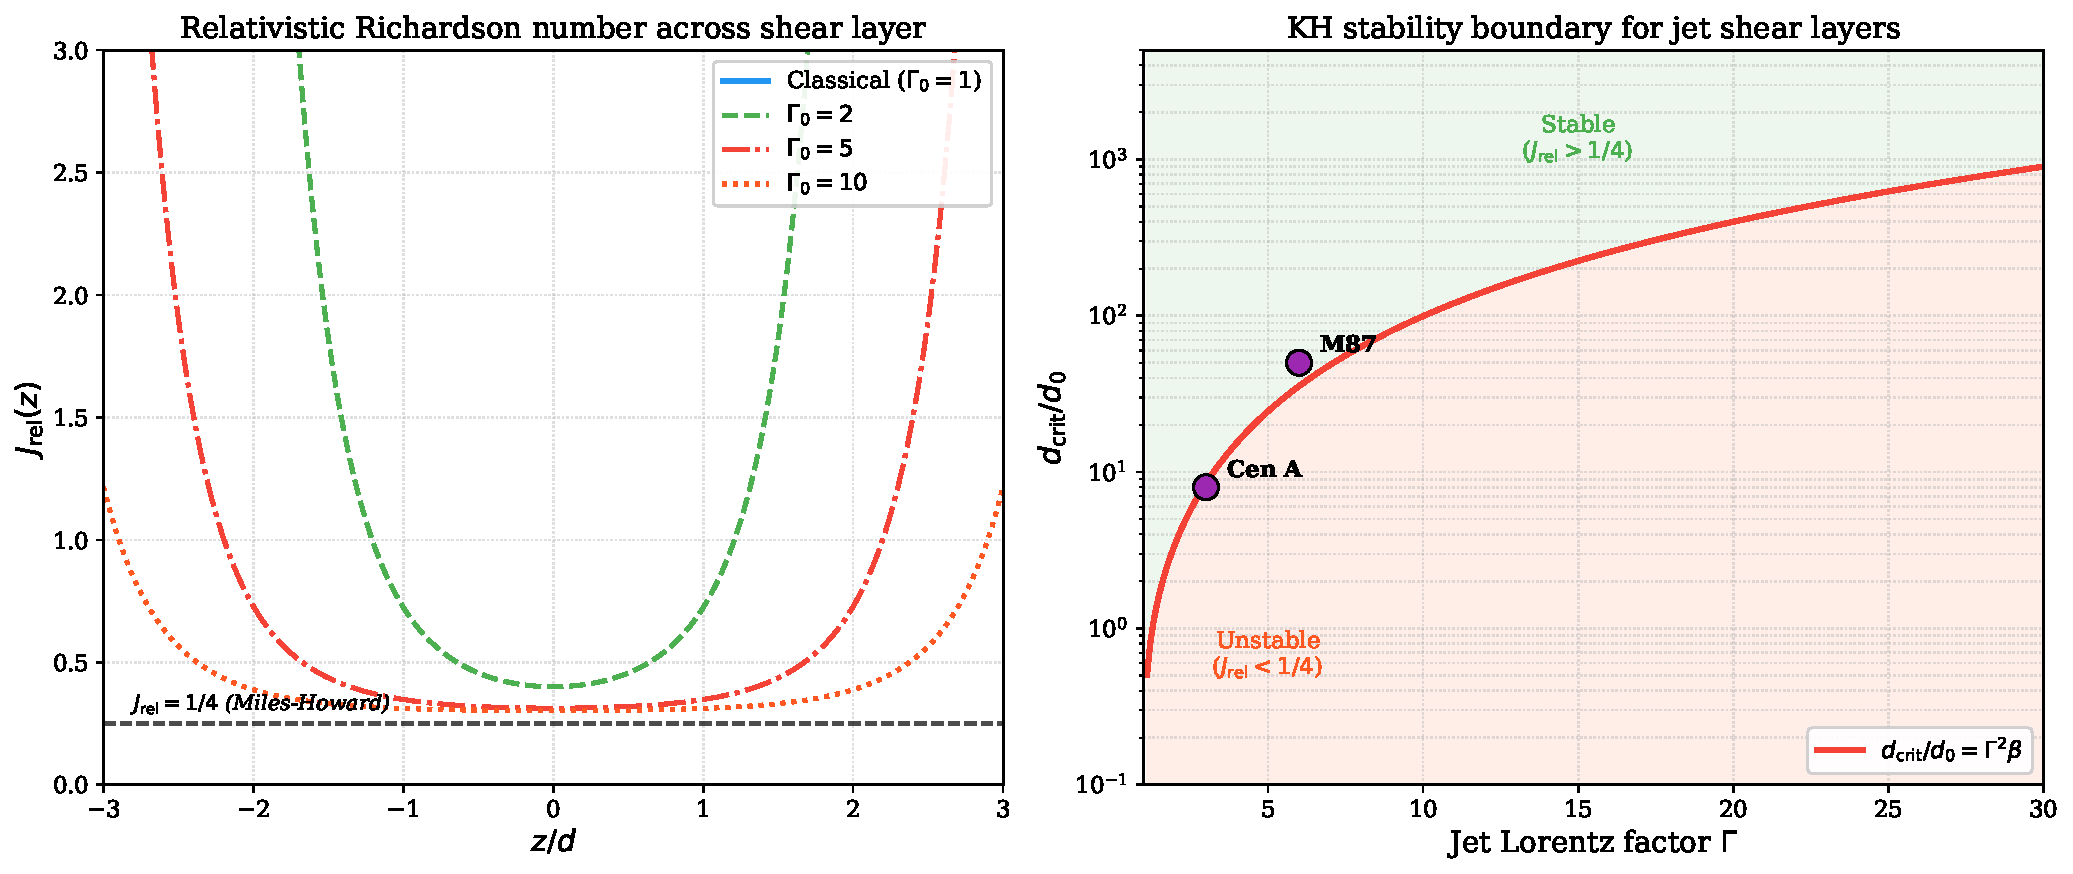
\includegraphics[width=0.95\textwidth]{plots/ch11/fig_miles_howard_ri_rel.pdf}
\caption{%
\textbf{Left:} Relativistic Richardson number $J_{\mathrm{rel}}(z)$
across a $\tanh$ shear layer for $\Gamma_0 = 1$ (classical), 2, 5, and 10.
The dashed line marks the Miles--Howard threshold $J_{\mathrm{rel}} = 1/4$.
\textbf{Right:} Critical shear-layer width (normalised) vs.\ $\Gamma$
for stability, with observed positions of M87 and Cen~A marked.
}
\label{fig:miles-howard-ri-rel}
\end{figure}
